\section{Results}
In our experiments, we aimed to answer three key questions:  
(a) How accurate is the model-based prediction system?  
(b) How agile is the whole-body control policy designed for table tennis?  
(c) When integrated, how effectively can the system return the ball and even play against human or humanoid opponents in the real world?

\begin{figure*}
    \centering
    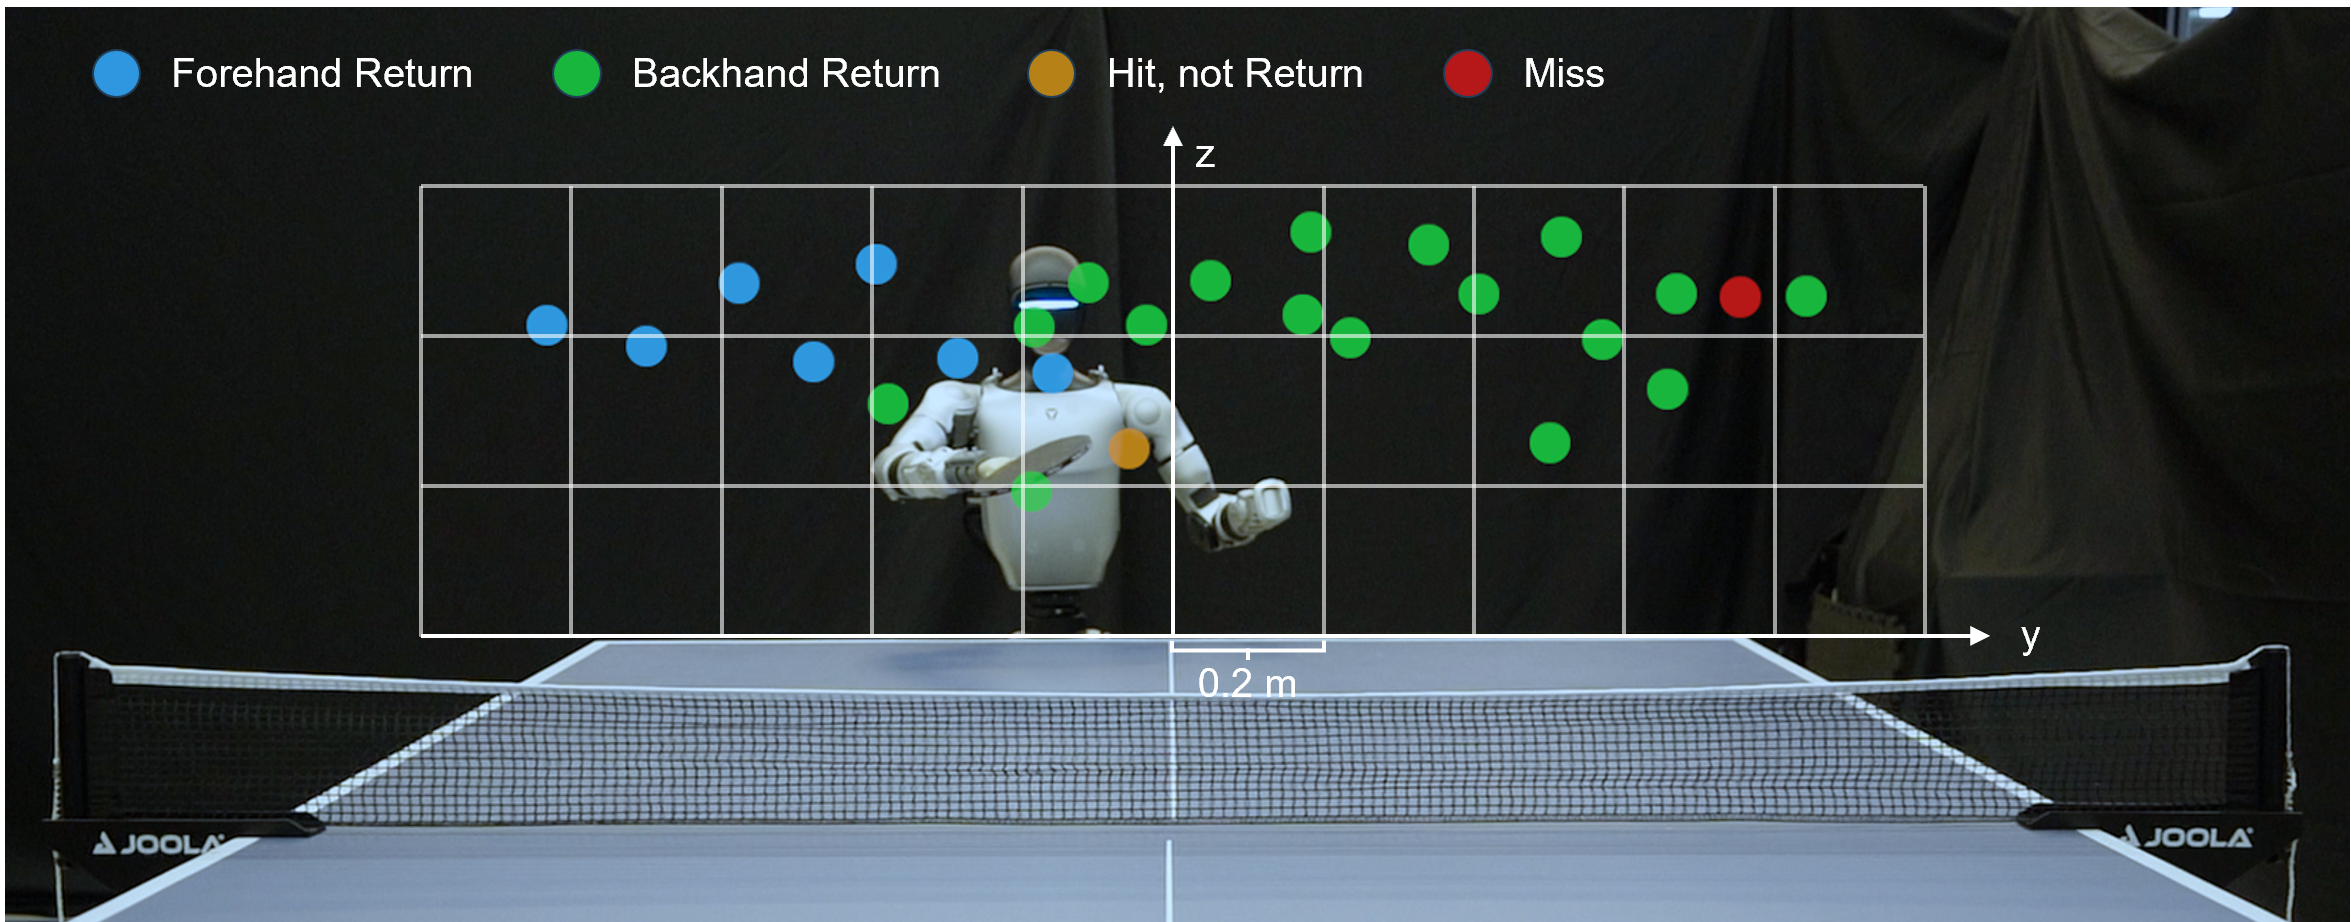
\includegraphics[width=\linewidth]{figures/succ_rate.png}
    \caption{\textbf{Return performance evaluation.} The results are displayed on a virtual hit plane, with each block side representing 0.2\,m. Of the 26 incoming balls distributed across the plane, the robot successfully returned 24 (blue: forehand strokes, green: backhand strokes), while 1 hit did not result in a return (orange) and 1 was a complete miss (red). This corresponds to a 96.2\% hit rate and a 92.3\% return rate.}
    \label{fig:succ_rate}
\end{figure*}

\subsection{Model-based Planner}

To evaluate the performance of the model-based planner, we collect 20 ball trajectories and compute the prediction errors for both the hitting position and strike time (Fig.~\ref{fig:prediction_error}). The errors decrease as the strike approaches, reaching zero at the moment of contact. This trend aligns with the intuition that longer prediction horizons accumulate larger errors. At 0.5\,s before the strike, the position prediction error falls below the critical threshold of 7.5\,cm, corresponding to the racket’s radius. At 0.3\,s before the strike, the time prediction error drops below 20 ms, equivalent to one control step of the policy. At 0.1\,s before the strike, both position and time errors reach minimal level. The consistently low error across the entire prediction process provides a stable command interface for the WBC policy and establishes a foundation for the overall accuracy of the system.


\subsection{Whole-Body Control}

We examine the relation between the initial distance from the desired base position $\hat{\mathbf{p}}_{\mathrm{base}}$ to the actual base position $\mathbf{p}_{\mathrm{base}}$ at the moment a new command is sampled, and the time required to reach within 1\,cm of $\hat{\mathbf{p}}_{\mathrm{base}}$ to evaluate the agility of the whole-body control policy. We collect 1000 roll-outs in simulation and discard 57 cases where the 1\,cm threshold is not reached, resulting in 943 valid data points and a success rate of 94.3\%. As shown in Fig.~\ref{fig:agility_test}, when the initial distance is less than $0.75$\,m, nearly all trials converge to within 1\,cm of $\hat{\mathbf{p}}_{\mathrm{base}}$ in less than 0.8\,s, which is shorter than the typical duration from command issuance to strike (0.86\,s), as described in Sec.~\ref{subsec:hmr}. This indicates that, in almost all cases, the robot successfully reaches the desired base position before the striking motion is completed. Moreover, convergence time increases monotonically with the initial distance, as expected. The statistical distribution is highly symmetric, with comparable convergence times for displacements in both the left and right directions. The results demonstrate the agility of the WBC policy in simulation.

In the real world, we observe that the policy consistently exhibits agile motions. As shown in Fig.~\ref{fig:side_jump}, the robot initially stands on the right side of the table. When the ball is directed toward the left side, it reacts quickly and, with a single step, moves across to return the ball rapidly. This prompt, one-step motion is enabled by commanding the base position. In contrast, when using velocity commands as in prior WBC approaches~\cite{cheng2024expressive}, the robot consistently performs slower, multi-step lateral movements. For the upper-body arm swing, training with human motion references produces striking behaviors that closely resemble human motions, including waist rotation during the hit, as demonstrated in Fig.~\ref{fig:hit_motion}.

\subsection{Real-World Experiments}
When we deploy our system, we throw 26 balls toward the robot, with their projections on the virtual hit plane spanning a wide area. The robot achieves 24 successful returns, misses 1 return after a hit, and completely misses 1 ball, corresponding to a 96.2\% hit rate and a 92.3\% return rate (Fig.~\ref{fig:succ_rate}). We also observe that the robot tends to use forehand strokes for balls incoming at $y < 0$ and backhand strokes for balls incoming at $y > 0$, which is consistent with human table tennis play.

Moreover, our humanoid can engage in extended play against human opponents, achieving rallies of up to 106 consecutive shots. This rally ends when the humanoid hits the ball into the net. Such a rally length exceeds that of casual human play, indicating that the humanoid not only tracks and returns the ball reliably but also maintains balance and readiness across successive strokes. The humanoid can even return human smashes with only 0.42\,s of reaction time from the opponent’s hit to the robot’s return. Furthermore, when two humanoids equipped with the same policy face each other, they can sustain continuous rallies in a fully autonomous match setting (Fig.~\ref{fig:teaser}).
